%%%%%%%%%%%%%%%%%%%%%%%%%%%%%%%%%%%%%%%%%
% University/School Laboratory Report
% LaTeX Template
% Version 3.1 (25/3/14)
%
% This template has been downloaded from:
% http://www.LaTeXTemplates.com
%
% Original author:
% Linux and Unix Users Group at Virginia Tech Wiki 
% (https://vtluug.org/wiki/Example_LaTeX_chem_lab_report)
%
% License:
% CC BY-NC-SA 3.0 (http://creativecommons.org/licenses/by-nc-sa/3.0/)
%
%%%%%%%%%%%%%%%%%%%%%%%%%%%%%%%%%%%%%%%%%

%----------------------------------------------------------------------------------------
%	PACKAGES AND DOCUMENT CONFIGURATIONS
%----------------------------------------------------------------------------------------

\documentclass{article}

\usepackage{graphicx} % Required for the inclusion of images
\usepackage{natbib} % Required to change bibliography style to APA
\usepackage{amsmath} % Required for some math elements 
\usepackage{amsthm}
\usepackage[hyphens]{url}
\usepackage{hyperref}
\usepackage{subcaption}
\usepackage{float}
\usepackage{array}
\usepackage{amssymb}
\usepackage{calrsfs}
\usepackage{pgfplots}
\pgfplotsset{width=10cm,compat=1.9}
\usepackage{bytefield}


\setlength\parindent{0pt} % Removes all indentation from paragraphs

\newtheorem*{remark}{Theorem}
\newtheorem*{definition}{Definition}

%----------------------------------------------------------------------------------------
%	DOCUMENT INFORMATION
%----------------------------------------------------------------------------------------

\title{Homework \#5 \\Telegram vs WhatsApp Security \\[0.2em]\small{}CNS Course Sapienza} % Title and subtitle

\author{Riccardo \textsc{Prinzivalle}, 1904064} % Author name

\date{November 30, 2020} % Date for the report

\begin{document}

\maketitle % Insert the title, author and date

%----------------------------------------------------------------------------------------
%	SECTION 0
%----------------------------------------------------------------------------------------

\section{Homework Goal}

This homework contains a basic introduction to Telegram and WhatsApp security, then a comparison of their security protocols (\textbf{MTProto} and \textbf{Signal} respectively), some past development and technical issues/vulnerabilities, and what it is possible to find about current threat and vulnerabilities.

%----------------------------------------------------------------------------------------
%	SECTION 1
%----------------------------------------------------------------------------------------

\section{Telegram Security basics}

Telegram uses a security protocol called MTProto, developed by the telegram team. It is a symmetric encryption protocol based on 256-bit symmetric AES encryption, 2048-bit RSA encryption and Diffie–Hellman key exchange. The protocol is divided in 3 layers:

\begin{itemize}
	\item \textbf{High-level} component which defines the method whereby API queries and responses are converted to binary messages.
	\item  \textbf{Cryptographic/authorization} layer which defines the method used to encrypt messages prior to being transmitted through the transport protocol.
	\item  \textbf{Transport} component, which defines the method for the client and the server to transmit messages over some other existing network protocol.
\end{itemize}

Let's analyze in the details every section. The high level component sees a client and a server exchanging messages inside a session, which is identified by a user key identifier (a particularity, the session is attached to the client instead of standard protocols such as http/s or tcp). The client can instantiate different connections to the server (the practicality of Telegram stands in the fact that one can open different sessions on many devices such as browsers without having to log in many times once one have the session active), and messages can be sent from one connection to the other and everything is synchronized server side. The low level message structure can be seen in fig. \ref{fig:tel_pack}.

\begin{figure}[H]
	\centering
	\begin{bytefield}[bitwidth=0.55em]{64}
		\bitheader{0,4,8,12,16,20,24,28,32,36,40,44,48,52,56,60,64} \\
		\begin{rightwordgroup}{encryption \\ header}
			\bitbox{64}{key identifier} \\
			\wordbox[tlr]{1}{message key} \\
			\wordbox[blr]{1}{128 bit} 
		\end{rightwordgroup} \\
		\\
		\begin{rightwordgroup}{message \\ header}
			\bitbox{64}{message identifier} \\
			\bitbox{64}{server salt}
		\end{rightwordgroup}
		\\
		\begin{rightwordgroup}{message \\ payload}
			\bitbox{32}{message sequence number} & \bitbox{32}{message length} \\
			\wordbox[tlr]{3}{message body (32 bit multiple)} \\
			\bitbox[blr]{32}{}
			& \bitbox{32}{type dependent parameters}
		\end{rightwordgroup} \\
	\end{bytefield}
	\caption{Telegram simplified packet structure}
	\label{fig:tel_pack}
\end{figure}

The message header is fixed for every message, the types of parameters does not change, and they are used by the encryption part, like message identifier and server salt.\newline
To be mentioned, all number are saved as little endian, with the exception of large numbers, such as those needed by RSA and DH which are stored as big endian due to openSSL compatibility.\newline
The encryption stuff can be identified in the upper part fig. \ref{fig:tel_pack}, it is added at the end of encryption as header of the encrypted message. The message is encrypted using a 256-bit key constituted by the message key and the user key and the encryption is performed with AES-256. The message key is defined as the hash using SHA256 on the message body, and taking the 128 middle resulting bits. The user key is generated from the authorization key: it is created once, when the client is first run on the device, and never changes, so this will expose all messages if that key is stolen (even from the device or from server side); different counter measures can be taken: 

\begin{itemize}
	\item Use session keys generated at every session using the Diffie Hellman exchange protocol
	\item Store the keys on the device and protect them with a password
	\item Protect all stored and cached data of the device with a password
\end{itemize}

All these measures cannot protect the user in the case where is the server that is violated or some government agency ask the keys for terrorism prevention (as example). The complete encryption scheme for every message can be seen in fig \ref{fig:MTProto}.

\begin{figure}[H]
	\centering
	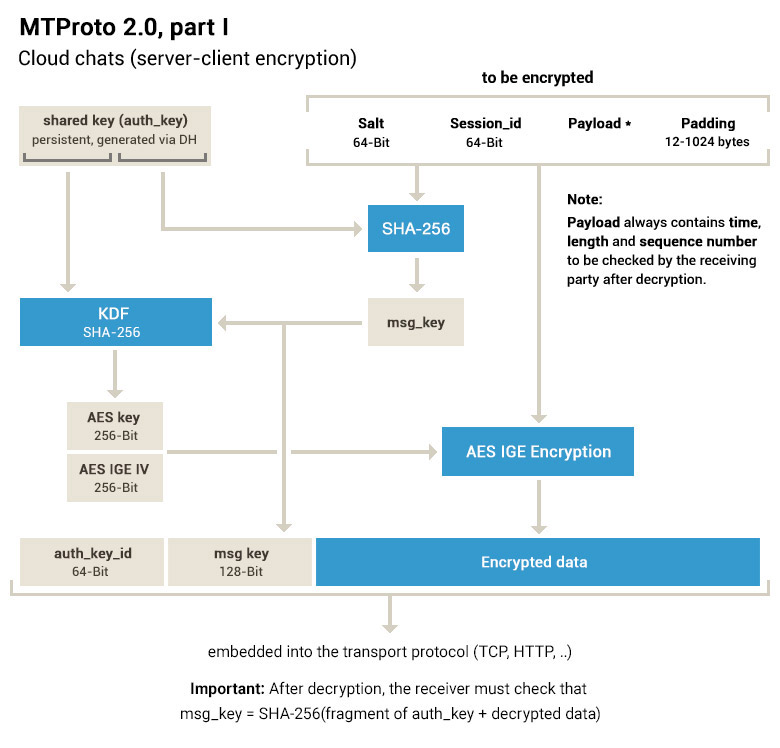
\includegraphics[width=0.9\textwidth]{images/mt_p1.jpg}
	\caption{MTProto}
	\label{fig:MTProto}
\end{figure}

The message identifier field is strictly related to time on the sender machine, and the receiver checks it with its time, so if there is a time divergence on sender or receiver message (here it is intended client/server communication and vice versa) then the receiver start to drop messages: in this case, the server (even if its time is not correct) will send a service message asking the client to synchronize its time with the server one. The time synchronization is simply defined as storing the difference between server and client time on client side. If the synchronization fails then the client must start a new session to continue the communication.\newline
The transport layer encapsulated the encrypted message with a secondary protocol header depending on specification of the message contained in the header, this allows to obtain additional services such as \textit{quick ack} or \textit{transport error}. The effective transport then relies on existent transport layer protocols as TCP, websockets or HTTP/S.\newline
This section has been developed using \cite{MTProto} and \cite{tel_wiki} as references.

%----------------------------------------------------------------------------------------
%	SECTION 3
%----------------------------------------------------------------------------------------

\section{WhatsApp Security Basics}

WhatsApp security relies on \textbf{Signal} protocol: it allows end-to-end encryption of every communication through the application. The protocol is based on the following steps:

\begin{itemize}
	\item Client registration and public keys exchange
	\item Encrypted session creation
	\item Message exchange using \textbf{Double Ratchet Algorithm} to generate a key for every message
\end{itemize}

When a new client is registered, some public keys are sent to the server who stores them: these keys are a \textit{public identity key}, a \textit{signed pre key} with its signature and a batch of \textit{one time pre keys}. These elements allow the server to uniquely identify a user identity.\newline
Every communication with a user is treated as an encrypted session: it is established at the first message exchanged and it does not change until no external factor changes the integrity of the session (this can happen due to a device change or an app reinstall). The session is created using the public keys of the receiver retrieved from the server and they are used to generate a master secret by "or" operation of different Diffie Hellman based on Elliptic Curves. The secret key is used by an hashed key derivation function to create a root key and some chain keys. If the recipient is not online at the time of the creation of the session, then the initiator includes the information to start the session with the first message sent, in order for the recipient to start the same encrypted session when he receives the messages.\newline
Every message sent through a session are encrypted by a message key using AES256 and HMAC-SHA256 for authentication. The message key changes for every message and it is ephemeral, so it is not possible to reconstruct an encrypted message from the session state. The key generation is based on the \textbf{Double Ratchet Algorithm}: it is based on HMAC-SHA256 to generate the single message key from the ratchet chain key and on the association of ECDH and HKDF to generate the new chain key and root key for the next message (these steps guarantee forward secrecy). This mechanism can cause delay in the messages and shift on the order of the original messages, but since every message is encrypted separately, it is not a problem. The Double ratchet scheme can be seen in fig. \ref{fig:doubleratchet}; the letters A and B are the message sent by Alice or Bob, and the number is the number of the message sent by one of them.

\begin{figure}[t]
	\centering
	\begin{subfigure}[b]{0.5\textwidth}
		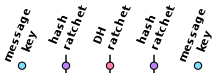
\includegraphics[width=1\linewidth]{images/doubleratchet_synt_header.png}
	\end{subfigure}
	\begin{subfigure}[b]{0.5\textwidth}
		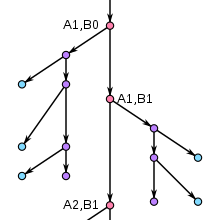
\includegraphics[width=1\linewidth]{images/doubleratchet_synt.png}
	\end{subfigure}
	\caption{Double Ratchet \cite{dr_scheme}}
	\label{fig:doubleratchet}
\end{figure}

The user can verify the end-to-end encryption keys to avoid a man-in-the-middle attack, the verification can be performed either by a QR code or by a 60 digit number, that the users must compare with the keys stored on their device to ensure no attack has been performed.\newline 
For what concerns the transport layer, WhatsApp uses the \textbf{Noise} protocol framework: this provides long time connections between the clients and the servers based on \textit{noise pipes} with Curve25519, AES-GCM, and SHA256.\newline
Unfortunately, I was not able to find images like fig. \ref{fig:MTProto} for WhatsApp; this is due to the nature of \textbf{Signal} protocol, which subdivides every step of security into separated applications, such as the Double Ratchet of fig. \ref{fig:doubleratchet}. This section is based on \cite{what_tech_paper}, \cite{what_medium}, \cite{what_wiki} and \cite{signal}.

%----------------------------------------------------------------------------------------
%	SECTION 4
%----------------------------------------------------------------------------------------

\section{Protocols comparison}

This section contains some comparisons of both protocols, evidentiating some key aspect and vulnerabilities. \newline
It can be easily seen that telegram hides some big hole in security: the first problem is its usability, to guarantee that, telegram uses session attached to the clients, so the session decades only when the client closes it; in addition one can enter a past session which is still open in a device just by going to the site and the cookies will automatically log in the user to that session. Furthermore, everything sent with telegram (messages, media, links and files) is all stored on server side, this will facilitate the user to obtain everything from every device where he is logged in, but if it is easier for the end user also someone interested in that data will gain access in easier way. Another problem is that all messages are encrypted with a key derived from the authorization key: this key rarely changes, and exposes all messages in the cases it is stolen from a device, this is due to the structure of the key derivation, from which it is possible to decrypt every message once it is stolen.\newline
Furthermore, not all the chats are end-to-end encrypted, only secret chats have this privilege, so a basic user does not know this difference and he generally uses the standard chats, so his message can be decrypted server side: this introduces another problem of telegram, the server keys are known to the telegram organization, and as it will be seen in the next sections, it is a big trouble for the end user. In addition to that, the server implementation is closed source, so the effectively security of server side cannot be verified by the user or others neutral entities.\newline
Another problem is based on the time synchronization: if one of server or client have a different time, then the messages will began to be discarded, and since it is always the server who send the reference time for the synchronization, if a server is compromised, then an attacker can instantiate a DOS attack.\newline
WhatsApp instead has better masked his security holes. This app uses end-to-end encryption for every communication, a problem stands in the initialization of the encryption: the first messages shared with a new chat/user contains the informations to start the encrypted session, so if the messages are intercepted by someone else other than the effective receiver, one can in some way listen to the session from that moment on, since the session keys changes only for rare events, such as app reinstall or device changes. An attacker can also become active if he has the session keys and inject false messages in the session. For what concerns the usability on browser, the opened session expires after some small time of inactivity.\newline
In both cases the message key changes for every message, WhatsApp uses a more reliable message key generation, but if the session key is stolen then it is possible to rebuild every message key. If a message key is stolen, then only the associated message can be decrypted, but none of past and future message keys can be derived from another message key.\newline
For the transport layer, Telegram uses a proprietary protocol on top of the standard ones, so transport security relies on the security of open transport layer protocols. WhatsApp instead relies completely on the Noise Protocol, which is open as in the other case of Telegram.\newline
WhatsApp has both client and server closed source, so it has the same problem of Telegram when it comes about security verification by third party neutral entities.\newline
The problem on both apps is that they are ruled by companies whose policies are not so secure: in one case the Telegram Messenger Inc has doubtly policies \cite{tel_policy} and server keys are in their hand; on the contrary WhatsApp \cite{whats_policy} is in the hand of Facebook, not one of the clearest companies in the world.\newline
To recap, a small list of both protocols' problems:

\begin{itemize}
	\item both have some pieces closed source, so no security verification
	\item both protocols have problems with the initialization of the session, if the session keys are stolen then all the messages can be decrypted
	\item telegram has also problem worth time synchronization and server side encryption (the latter only for not secret chat) 
	\item both have problems with browser session, Telegram problem is a bit huge w.r.t. the WhatsApp counterpart
\end{itemize}

The comparison has taken in exam only the standard one-to-one chat, another analysis can comprehend also media, group chats and call/videocall security, which in the case of WhatsApp can be of big concerns \cite{what_security_threat}.
 
%----------------------------------------------------------------------------------------
%	SECTION 5
%----------------------------------------------------------------------------------------

\section{Past Evolution and Fixed Vulnerabilities}

The first app was WhatsApp, founded in 2009, at that time the app sent all the messages as plaintext, the first form of cryptography was added back in 2012, but it wasn't end-to-end-encryption and it was considered broken after few time \cite{what_threat}. Many securities and government entities demonstrated their doubts about WhatsApp security issues during the period from 2012 to 2015 \cite{what_threat}, and this pushed WhatsApp to implement some better form of security. So end-to-end encryption was introduced only in 2014 \cite{what_ete} when WhatsApp joins Open Whisper Systems; the encryption is practically implemented using Signal protocol. Some time previous of WhatsApp e-t-e encryption was introduced, Telegram was founded in Russia (2013). The problem with Telegram is that it uses a closed source encryption protocols, which has been  demonstrated to not be fully secure \cite{MT_insecure}, and this protocol is still use today's. One year after Telegram foundation, their creators affirm that all the source code will eventually be released, but only the client code was released, the server side is still closed source. To overcome this problem, the Telegram company organized two cryptoanalysis contests \cite{contest1} \cite{contest1} to prove that its cryptography is secure enough, but suspiciously no one was able to break any vulnerabilities of the messaging app (it is generally suspected that the results are not completely clear and misleading). \newline
In 2016 Telegram suffers an attack on the method used to authenticate users \cite{2factor}, the attack consists on the SMS spoofing on the messages used to authorize a new session, so it is not an attack performed against Telegram itself, but since it relies on this method for the authentication, then it is not secure. Today's it is suggested to use a 2-factor authentication to overcome this problem. During the years, many more attacks like this were perpetrated against activists and government members by exploiting SMS vulnerabilities for authentication or inserting malwares inside the device of the victims \cite{brasil_leak} \cite{russia_leak} \cite{telegram_gate}. Another episode comprehend a big leak of Iranian Telegram accounts, together with private information, but also in this case the leak was due to problems not directly attributable to Telegram app itself, one of the method implied the exploit of Telegram desktop, but the other relied on device hacking or phishing techniques \cite{iran_leak}. \newline
The WhatsApp e-t-e encryption needed two years to be fully implemented, and only in 2016 every form of communication made through the app is fully encrypted, and end users can verify each other keys as seen in previous sections.\newline
To simplify friends' contact discovery, both application send to the server a copy of the mobile entire addresses' book, it is not clear how securely this data are sent and stored on the server, but form privacy policies, it is supposed that they don't use an enough high level of security compliant with different states regulator's policies.\newline 
During the years, WhatsApp has suffered from several security bugs, such as ack crash \cite{ack_crash} and the web app bugs \cite{what_web}. It is not clear if these bugs are effectively fixed as today.\newline
WhatsApp credibility on policies has been completely doubted after the Facebook acquisition in 2014 and later policies updated by the Facebook company.\newline
In 2017 WhatsApp experienced a controversy with an article published on The Guardian, which discloses some vulnerabilities in e-t-e encryption, but both WhatsApp and Open Whisper Systems denied these vulnerabilities; despite these threat not being recognized officially, WhatsApp introduced a two-factor authentication and verification (this feature was already in beta, but the timing seems suspect) \cite{what_threat}.\newline
For further readings see Wikipedia references for both applications \cite{tel_wiki} and \cite{what_wiki}

%----------------------------------------------------------------------------------------
%	SECTION 6
%----------------------------------------------------------------------------------------

\section{Current Vulnerabilities and Security Threats}

As seen in previous section, till today's, no attack perpetrated against the Telegram application itself are known, but what is not clear is how much the Telegram organization has access to every data exchanged on their servers: many episodes of censorship has been documented \cite{china_cen}, \cite{honk_cen}, \cite{bahrain_cen}, \cite{pakistan_cen}, \cite{india_cen}, \cite{russia_cen} and \cite{iran_cen}; in different places among these, the Telegram company was pressured to disclose the server encryption key, or to loose the encryption algorithm, as happened in \cite{usa_weak}.\newline
As of today, Telegram still has its server side source code private, this introduces doubts over thrusting the company about the effective data security, since if the server keys are accessible by the company, everyone can breach the server and obtain them or it is directly the company spying over its users, but it is not effectively documented, just hypothesis of future and current threat over our privacy.\newline
A point in favor of WhatsApp is that both encryption protocol and messaging protocols are accessible and open source, so a technical end user or some third parties can publicly verify the security of this app, while the effectively client and server implementation are closed source, so the app is only based on these open source projects, but at the end it is a closed source application, so some vulnerabilities can be discovered slower than in open source contest.\newline
In 2019 it was found a possibility to install a spyware through WhatsApp by making a call which did not even need answer; the company introduced a bounty hunter on the bug but as of today it seems to still be an issue \cite{what_threat}.\newline
As stated in \cite{new_EU}, a new EU directive says that in the nearest future, all the European External Action Service (EEAS) will rely on a new secret communication application, not currently released instead of using WhatsApp and Signal: this brings up new problems, such as the open sourceness of the project (probably not), and consequently the real level of security provided by this new app (as already know, security by obfuscation is never a good idea); at least the data EU diplomacy chat will remains in the hand of a government agency and not in some extra company whose policies are not that clear.\newline
Other threats can arise from metadata \cite{threat}: this article may seem referring to Telegram only, instead it introduces also WhatsApp, Signal and iMessage vulnerabilities caused by metadata which remains on the sender device and sometimes are sent in clear to the server as information on identification and for other purposes. This exposes another WhatsApp problem (and of many other instant messaging applications): the chat backups are clearly stored on the user device, so if it is compromised, at the end of the day an attacker can easily access all the chat present in the backup.\newline
Even if the application are "secure" from computer point of view, there is always the human factor which weakens all security levels: a possible threat is to try to access the user's account and then steal the two-factor code by social engineering techniques, as stated in \cite{6ditigs_hack}.

%----------------------------------------------------------------------------------------
%	SECTION 7
%----------------------------------------------------------------------------------------

\section{Conclusion}

%TODO add send dunes meme

After this brief introduction on elliptic curves, it is obvious why they have been widely adopted in many cases of asymmetric encryption: they use less bits for the same level of security, so are more efficient to compute and their base concepts are easier to visualize. As suggested on section , EC can be easily used in hybrid encryption scheme, in the key exchange phase.
%----------------------------------------------------------------------------------------
%	BIBLIOGRAPHY
%----------------------------------------------------------------------------------------

\bibliographystyle{abbrv}

\bibliography{biblio}

%----------------------------------------------------------------------------------------


\end{document}
